\documentclass[tikz,border=10pt]{standalone}
% Shared look for every TikZ diagram. Load with % Shared look for every TikZ diagram. Load with % Shared look for every TikZ diagram. Load with \input{../../tools/tikz-style.tex}
\usepackage[T1]{fontenc}
\usepackage{lmodern}
\renewcommand{\sfdefault}{lmr}  % diagrams use the same serif as the text
\usetikzlibrary{arrows.meta, positioning, shapes.geometric, calc, fit, backgrounds}
\definecolor{cblue}{HTML}{4C78A8}
\definecolor{corange}{HTML}{F58518}
\definecolor{cgreen}{HTML}{54A24B}
\definecolor{cred}{HTML}{E45756}
\definecolor{cpurple}{HTML}{B279A2}
\definecolor{cgrey}{HTML}{6B6B6B}
\tikzset{
  every picture/.style={font=\sffamily, line width=1.2pt},
  box/.style={draw=#1, fill=#1!12, rounded corners=4pt, align=center, inner sep=7pt, minimum height=1.1cm},
  box/.default=cgrey,
  arrow/.style={-{Stealth[length=3mm]}, draw=cgrey, line width=1.4pt},
  title/.style={font=\sffamily\bfseries\Large},
  note/.style={font=\sffamily\small, text=cgrey, align=center},
}
\AtBeginDocument{\hyphenpenalty=10000 \exhyphenpenalty=10000}

\usepackage[T1]{fontenc}
\usepackage{lmodern}
\renewcommand{\sfdefault}{lmr}  % diagrams use the same serif as the text
\usetikzlibrary{arrows.meta, positioning, shapes.geometric, calc, fit, backgrounds}
\definecolor{cblue}{HTML}{4C78A8}
\definecolor{corange}{HTML}{F58518}
\definecolor{cgreen}{HTML}{54A24B}
\definecolor{cred}{HTML}{E45756}
\definecolor{cpurple}{HTML}{B279A2}
\definecolor{cgrey}{HTML}{6B6B6B}
\tikzset{
  every picture/.style={font=\sffamily, line width=1.2pt},
  box/.style={draw=#1, fill=#1!12, rounded corners=4pt, align=center, inner sep=7pt, minimum height=1.1cm},
  box/.default=cgrey,
  arrow/.style={-{Stealth[length=3mm]}, draw=cgrey, line width=1.4pt},
  title/.style={font=\sffamily\bfseries\Large},
  note/.style={font=\sffamily\small, text=cgrey, align=center},
}
\AtBeginDocument{\hyphenpenalty=10000 \exhyphenpenalty=10000}

\usepackage[T1]{fontenc}
\usepackage{lmodern}
\renewcommand{\sfdefault}{lmr}  % diagrams use the same serif as the text
\usetikzlibrary{arrows.meta, positioning, shapes.geometric, calc, fit, backgrounds}
\definecolor{cblue}{HTML}{4C78A8}
\definecolor{corange}{HTML}{F58518}
\definecolor{cgreen}{HTML}{54A24B}
\definecolor{cred}{HTML}{E45756}
\definecolor{cpurple}{HTML}{B279A2}
\definecolor{cgrey}{HTML}{6B6B6B}
\tikzset{
  every picture/.style={font=\sffamily, line width=1.2pt},
  box/.style={draw=#1, fill=#1!12, rounded corners=4pt, align=center, inner sep=7pt, minimum height=1.1cm},
  box/.default=cgrey,
  arrow/.style={-{Stealth[length=3mm]}, draw=cgrey, line width=1.4pt},
  title/.style={font=\sffamily\bfseries\Large},
  note/.style={font=\sffamily\small, text=cgrey, align=center},
}
\AtBeginDocument{\hyphenpenalty=10000 \exhyphenpenalty=10000}

\begin{document}
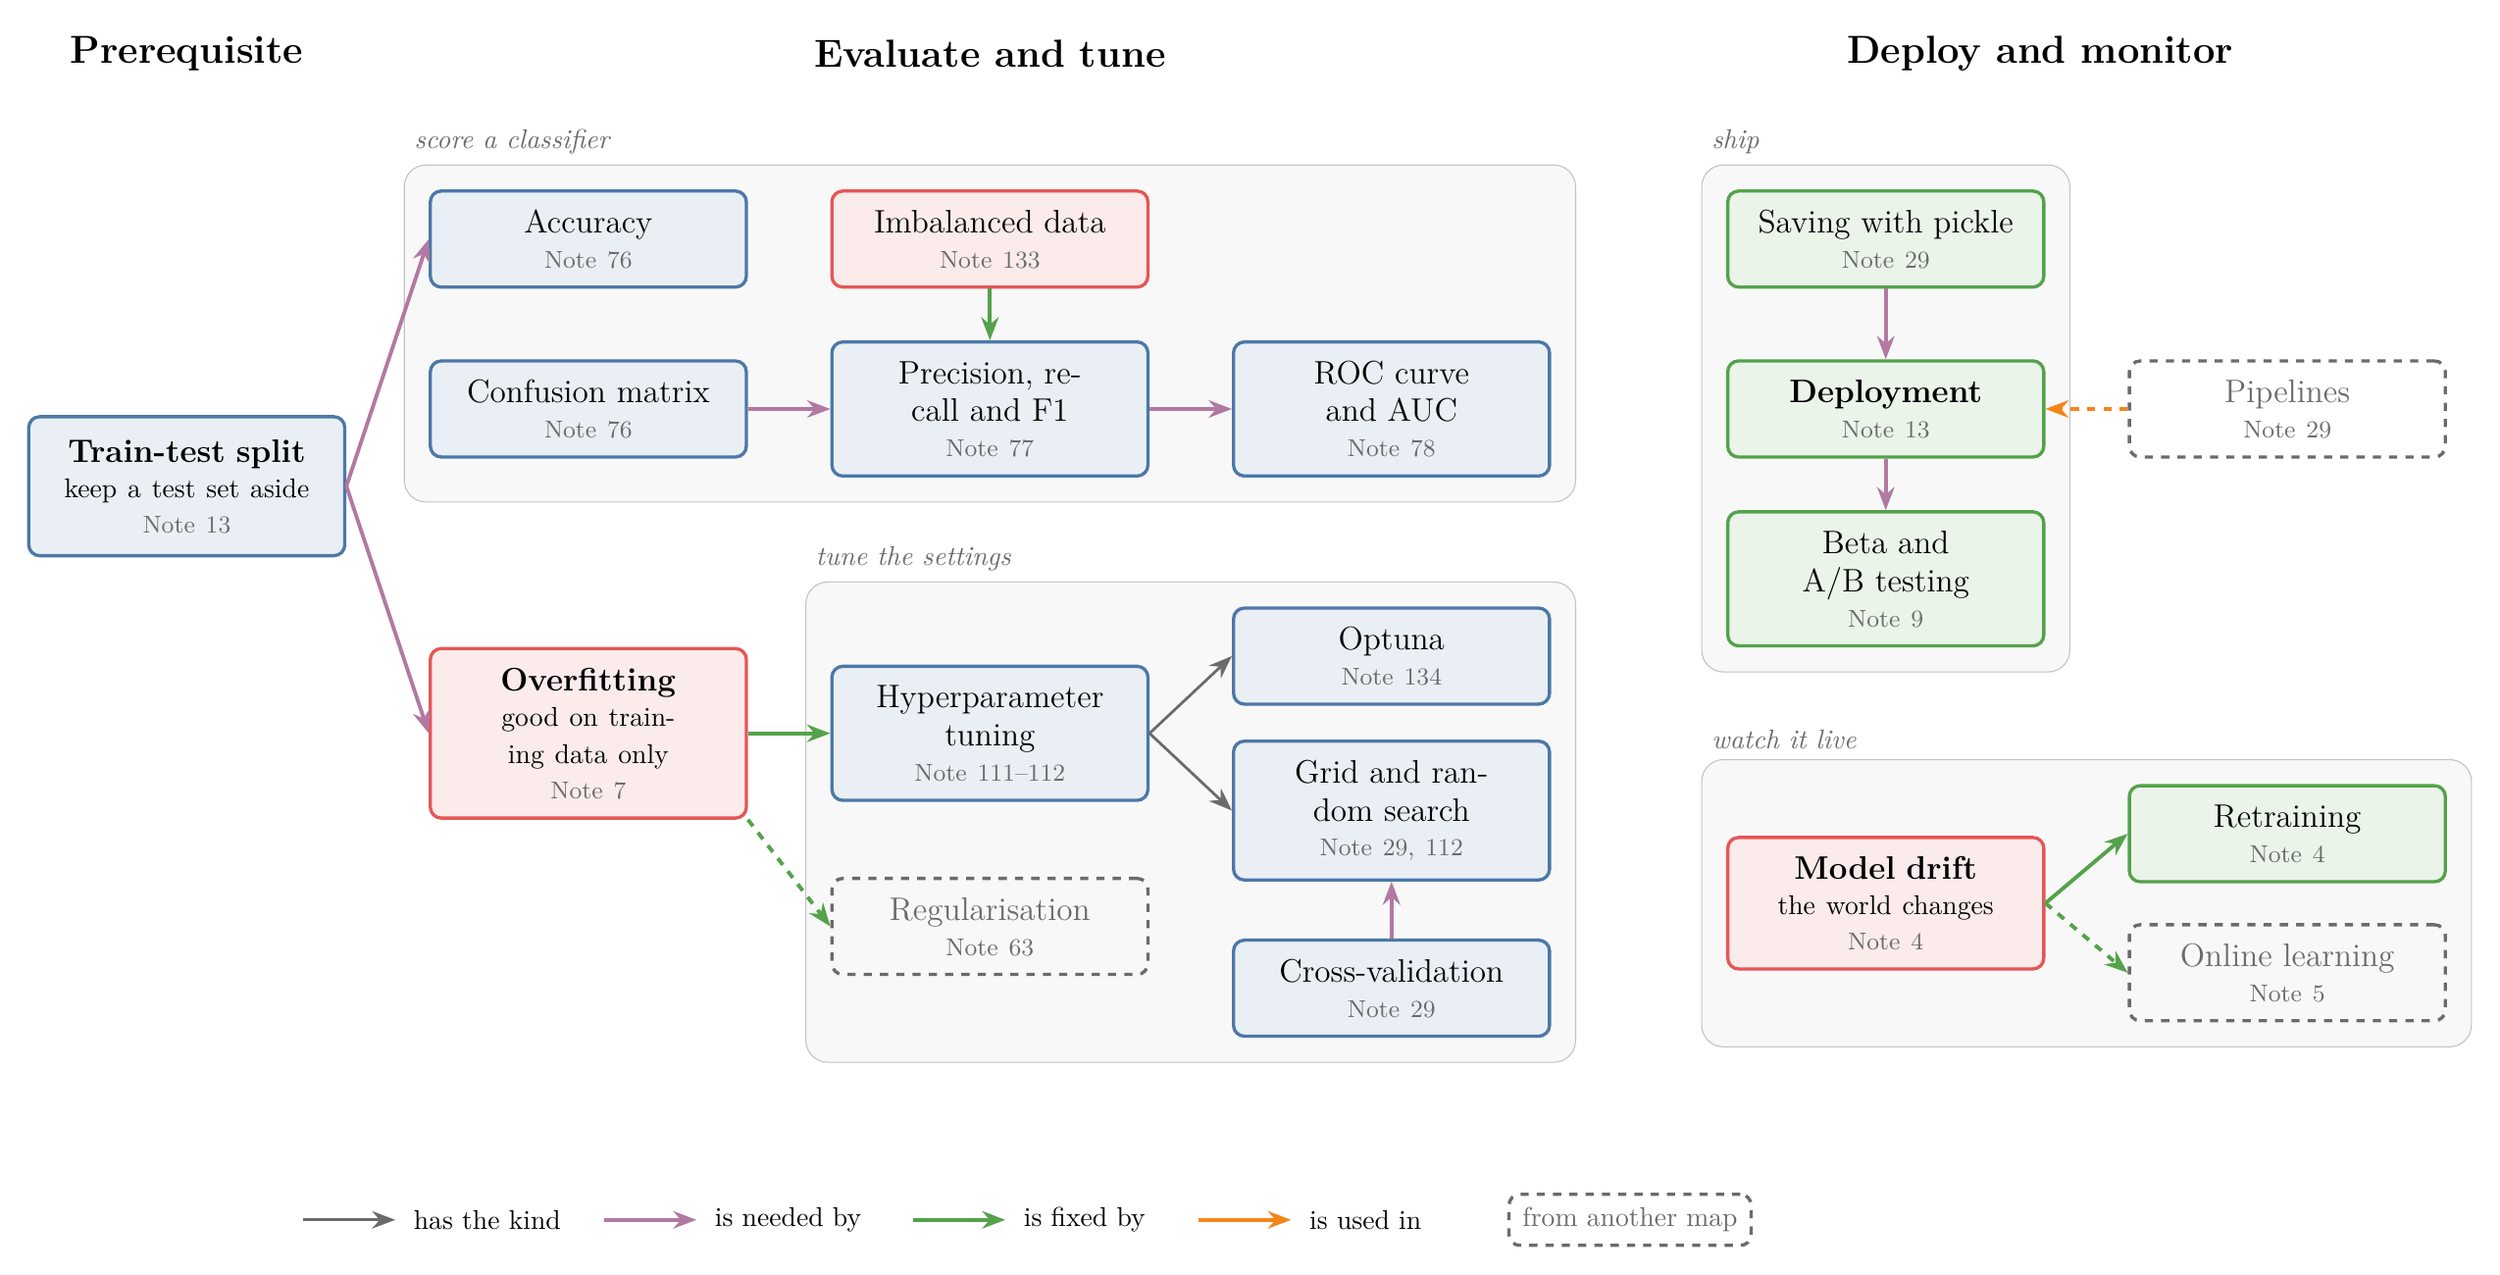
\begin{tikzpicture}[
    every node/.append style={font=\sffamily\large},
    con/.style={box=cblue, text width=3.6cm},
    prob/.style={box=cred, text width=3.6cm},
    ship/.style={box=cgreen, text width=3.6cm},
    prev/.style={draw=cgrey, dashed, rounded corners=4pt, align=center, inner sep=7pt, text=cgrey, text width=3.6cm, minimum height=1.1cm},
    group/.style={draw=cgrey!40, fill=cgrey!5, rounded corners=8pt, inner sep=9pt},
    gname/.style={font=\sffamily\normalsize\itshape, text=cgrey, anchor=south west},
    kindof/.style={arrow, draw=cgrey, line width=1pt},
    needs/.style={arrow, draw=cpurple},
    fixes/.style={arrow, draw=cgreen},
    usedin/.style={arrow, draw=corange},
  ]
  \newcommand{\nt}[1]{\\[-1pt]{\small\color{cgrey}Note #1}}
  \node[title] at (0,12.2)    {Prerequisite};
  \node[title] at (10.4,12.2) {Evaluate and tune};
  \node[title] at (24,12.2)   {Deploy and monitor};

  \node[box=cblue, text width=3.6cm, minimum height=1.8cm] (split) at (0,6.6) {\textbf{Train-test split}\\[-1pt]{\normalsize keep a test set aside}\nt{13}};

  % score a classifier
  \node[con]  (acc) at (5.2,9.8)  {Accuracy\nt{76}};
  \node[con]  (cm)  at (5.2,7.6)  {Confusion matrix\nt{76}};
  \node[con]  (pr)  at (10.4,7.6) {Precision, recall and F1\nt{77}};
  \node[con]  (roc) at (15.6,7.6) {ROC curve and AUC\nt{78}};
  \node[prob] (imb) at (10.4,9.8) {Imbalanced data\nt{133}};
  \draw[needs] (split.east) -- (acc.west);
  \draw[needs] (cm) -- (pr);
  \draw[needs] (pr) -- (roc);
  \draw[fixes] (imb) -- (pr);

  % overfitting and tuning
  \node[prob] (over) at (5.2,3.4)  {\textbf{Overfitting}\\[-1pt]{\normalsize good on training data only}\nt{7}};
  \node[con]  (tune) at (10.4,3.4) {Hyperparameter tuning\nt{111--112}};
  \node[con]  (opt)  at (15.6,4.4) {Optuna\nt{134}};
  \node[con]  (grid) at (15.6,2.4) {Grid and random search\nt{29, 112}};
  \node[con]  (cv)   at (15.6,0.1) {Cross-validation\nt{29}};
  \node[prev] (reg)  at (10.4,0.9) {Regularisation\nt{63}};
  \draw[needs] (split.east) -- (over.west);
  \draw[fixes] (over) -- (tune);
  \draw[fixes, dashed] (over.south east) -- (reg.west);
  \draw[kindof] (tune.east) -- (opt.west);
  \draw[kindof] (tune.east) -- (grid.west);
  \draw[needs] (cv) -- (grid);

  % deploy and monitor
  \node[ship] (pick) at (22,9.8) {Saving with pickle\nt{29}};
  \node[ship] (dep)  at (22,7.6) {\textbf{Deployment}\nt{13}};
  \node[ship] (ab)   at (22,5.4) {Beta and A/B testing\nt{9}};
  \node[prev] (pipe) at (27.2,7.6) {Pipelines\nt{29}};
  \draw[needs] (pick) -- (dep);
  \draw[needs] (dep) -- (ab);
  \draw[usedin, dashed] (pipe) -- (dep);

  \node[prob] (drift) at (22,1.2)  {\textbf{Model drift}\\[-1pt]{\normalsize the world changes}\nt{4}};
  \node[ship] (retr)  at (27.2,2.1) {Retraining\nt{4}};
  \node[prev] (onl)   at (27.2,0.3) {Online learning\nt{5}};
  \draw[fixes] (drift.east) -- (retr.west);
  \draw[fixes, dashed] (drift.east) -- (onl.west);

  \begin{scope}[on background layer]
    \node[group, fit=(acc) (imb) (roc) (cm)] (g1) {};
    \node[group, fit=(tune) (opt) (cv)] (g2) {};
    \node[group, fit=(pick) (ab)] (g3) {};
    \node[group, fit=(drift) (retr) (onl)] (g4) {};
  \end{scope}
  \node[gname] at (g1.north west) {score a classifier};
  \node[gname] at (g2.north west) {tune the settings};
  \node[gname] at (g3.north west) {ship};
  \node[gname] at (g4.north west) {watch it live};

  % legend
  \begin{scope}[shift={(1.5,-2.9)}, every node/.style={font=\sffamily, anchor=west}]
    \draw[kindof] (0,0) -- (1.2,0);   \node at (1.3,0) {has the kind};
    \draw[needs] (3.9,0) -- (5.1,0);  \node at (5.2,0) {is needed by};
    \draw[fixes] (7.9,0) -- (9.1,0);  \node at (9.2,0) {is fixed by};
    \draw[usedin] (11.6,0) -- (12.8,0); \node at (12.9,0) {is used in};
    \node[draw=cgrey, dashed, rounded corners=4pt, inner sep=5pt, text=cgrey, anchor=west] at (15.6,0) {from another map};
  \end{scope}
\end{tikzpicture}
\end{document}
